\chapter{Requisiti}

\section{Requisiti funzionali}
Per la realizzare del sistema si necessita:
\begin{itemize}
	\item di un utente in possesso di uno smartphone con sistema operativo Android versione 4.3 o superiore;
	
	\item uno o più iBeacon;
	
	\item un ambiente chiuso (come una stanza) in cui disporre gli iBeacon.
\end{itemize}
Nello specifico, per non alterare la ricezione dei segnali inviati dagli iBeacon, questi devono essere disposti:
\begin{itemize}
	\item su pareti regolari a circa 1 metro da terra;
	
	\item lontano da apparecchi che emettono onde elettromagnetiche (ad esempio router wifi);
	
	\item al sicuro da raffiche di vento;
	
	\item in aree in cui non si frappongano oggetti o persone tra lo smartphone e l'iBeacon target.
\end{itemize}

\section{Requisiti funzionali secondari}
Per poter avere un feedback a schermo della distanza reale utente-iBeacon si necessita di:
\begin{itemize}
	\item una board Arduino UNO (o superiore);
	
	\item un sensore ultrasonico;
	
	\item cavi di collegamento maschio-femmina;
	
	\item un cavo USB da stampante;
	
	\item uno smartphone che supporti la tecnologia \href{https://it.wikipedia.org/wiki/USB_On-The-Go}{\textbf{USB OTG (\textit{On-The-Go})}}\footnote{USB OTG - \url{https://it.wikipedia.org/wiki/USB_On-The-Go}}
	
	\item un cavo USB OTG.
\end{itemize}

%\section{Requisiti non funzionali}
%???

\section{Analisi dei requisiti}
\subsection{Casi d'uso}
\begin{figure}[ph]
	\centering
	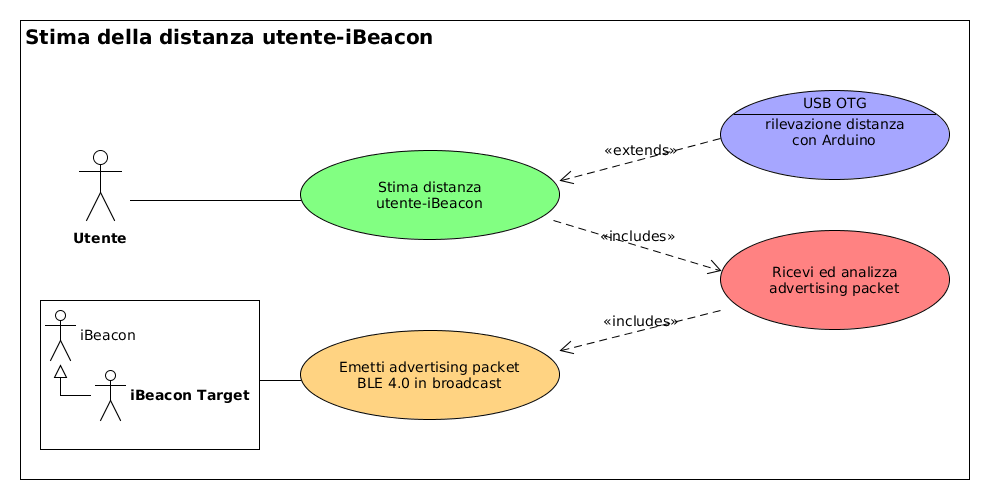
\includegraphics[scale=.45]{img/uml/use_case/use_case1}
	\caption[Use case - Stima della distanza utente-iBeacon]{Use case - Stima della distanza utente-iBeacon}
	\label{fig:usecase}
\end{figure}

\subsection{Scenari}

\subsubsection{\underline{Scenario classico}}
Nello scenario classico l'utente utilizza l'app per scansionare l'ambiente alla ricerca di iBeacon e leggere delle informazioni a schermo.

Nello specifico in questo scenario:
\begin{itemize}
	\item Si considera un utente in una stanza con uno smartphone Android in mano.
	
	\item La stanza in questione può presentare uno o più iBeacon disposti sui muri ad un'altezza di circa 1 metro dal suolo.
	
	\item Sullo smartphone viene avviata l'app.
	
	\item Nel caso in cui la radio Bluetooth dello smarphone fosse spenta o si dovesse spegnere, l'app stessa la accenderà/riaccenderà indicando all'utente l'avvenuto switch.
	
	\item L'utente preme su un bottone per avviare la scansione degli iBeacon presenti.
	
	\item Se vengono rilevati iBeacon corrispondenti con la lista di indirizzi MAC presente nell'app, allora viene caricata una lista di informazioni a schermo (\textit{friendly name}, immagine, distanza stimata, ecc\dots).
\end{itemize}

\subsubsection{\underline{Scenario classico avanzato}}
\begin{itemize}
	\item Una volta che l'utente ha visualizzato l'iBeacon di suo interesse (detto \textit{target}), lo seleziona dalla lista facendo click sull'item corrispondente.
	
	\item A questo punto all'utente vengono proposti solo i dettagli relativi al target, isolandoli dagli altri.
	
	\item In questa sezione l'utente potrebbe visualizzare un feedback della distanza reale (se tutte le condizioni a contorno sono soddisfatte) in metri.
	
	\item Trascinando il dito da destra a sinistra all'utente viene proposta un'altra area ancora più dettagliata dove è possibile mettere a confronto le varie stime della distanza (filtrata, non filtrata e reale se presente), in dei grafici realizzati in tempo reale.
\end{itemize}
